%%%%%%%%%%%%%%%%%%%%%%%%%%%%%%%%%%%%%%%%%
% Beamer Presentation
% LaTeX Template
% Version 1.0 (10/11/12)
%
% This template has been downloaded from:
% http://www.LaTeXTemplates.com
%
% License:
% CC BY-NC-SA 3.0 (http://creativecommons.org/licenses/by-nc-sa/3.0/)
%
%%%%%%%%%%%%%%%%%%%%%%%%%%%%%%%%%%%%%%%%%

%----------------------------------------------------------------------------------------
%	PACKAGES AND THEMES
%----------------------------------------------------------------------------------------

\documentclass{beamer}

\mode<presentation> {

% The Beamer class comes with a number of default slide themes
% which change the colors and layouts of slides. Below this is a list
% of all the themes, uncomment each in turn to see what they look like.

%\usetheme{default}
%\usetheme{AnnArbor}
%\usetheme{Antibes}
%\usetheme{Bergen}
%\usetheme{Berkeley}
%\usetheme{Berlin}
%\usetheme{Boadilla}
\usetheme{CambridgeUS}
%\usetheme{Copenhagen}
%\usetheme{Darmstadt}
%\usetheme{Dresden}
%\usetheme{Frankfurt}
%\usetheme{Goettingen}
%\usetheme{Hannover}
%\usetheme{Ilmenau}
%\usetheme{JuanLesPins}
%\usetheme{Luebeck}
%\usetheme{Madrid}
%\usetheme{Malmoe}
%\usetheme{Marburg}
%\usetheme{Montpellier}
%\usetheme{PaloAlto}
%\usetheme{Pittsburgh}
%\usetheme{Rochester}
%\usetheme{Singapore}
%\usetheme{Szeged}
%\usetheme{Warsaw}

% As well as themes, the Beamer class has a number of color themes
% for any slide theme. Uncomment each of these in turn to see how it
% changes the colors of your current slide theme.

%\usecolortheme{albatross}
%\usecolortheme{beaver}
%\usecolortheme{beetle}
%\usecolortheme{crane}
\usecolortheme{dolphin}
%\usecolortheme{dove}
%\usecolortheme{fly}
%\usecolortheme{lily}
%\usecolortheme{orchid}
%\usecolortheme{rose}
%\usecolortheme{seagull}
%\usecolortheme{seahorse}
%\usecolortheme{whale}
%\usecolortheme{wolverine}

%\setbeamertemplate{footline} % To remove the footer line in all slides uncomment this line
%\setbeamertemplate{footline}[page number] % To replace the footer line in all slides with a simple slide count uncomment this line

%\setbeamertemplate{navigation symbols}{} % To remove the navigation symbols from the bottom of all slides uncomment this line
}

\usepackage{graphicx} % Allows including images
\usepackage{booktabs} % Allows the use of \toprule, \midrule and \bottomrule in tables
\usepackage{mathrsfs}  
\usepackage{verbatim} 

%----------------------------------------------------------------------------------------
%	TITLE PAGE
%----------------------------------------------------------------------------------------

\title[VE216]{VE216 Recitation Class 6} % The short title appears at the bottom of every slide, the full title is only on the title page

\author{ZHU Yilun} % Your name
\institute[SJTU] % Your institution as it will appear on the bottom of every slide, may be shorthand to save space
{
UM-SJTU Joint Institute \\ % Your institution for the title page
\medskip
\textit{VE216 SU20 Teaching Group} % Your email address
}
\date{2020 Summer} % Date, can be changed to a custom date e.g.:\today

\begin{document}

\begin{frame}
\titlepage % Print the title page as the first slide
\end{frame}

\begin{frame}
\frametitle{Overview} % Table of contents slide, comment this block out to remove it
\tableofcontents % Throughout your presentation, if you choose to use \section{} and \subsection{} commands, these will automatically be printed on this slide as an overview of your presentation
\end{frame}

%----------------------------------------------------------------------------------------
%	PRESENTATION SLIDES
%----------------------------------------------------------------------------------------

%------------------------------------------------
\section{Chapter 4: Fourier Transform}
%------------------------------------------------

\subsection{FS vs FT}

\begin{frame}
    \frametitle{FS vs FT: for periodic signal}
    \begin{figure}
        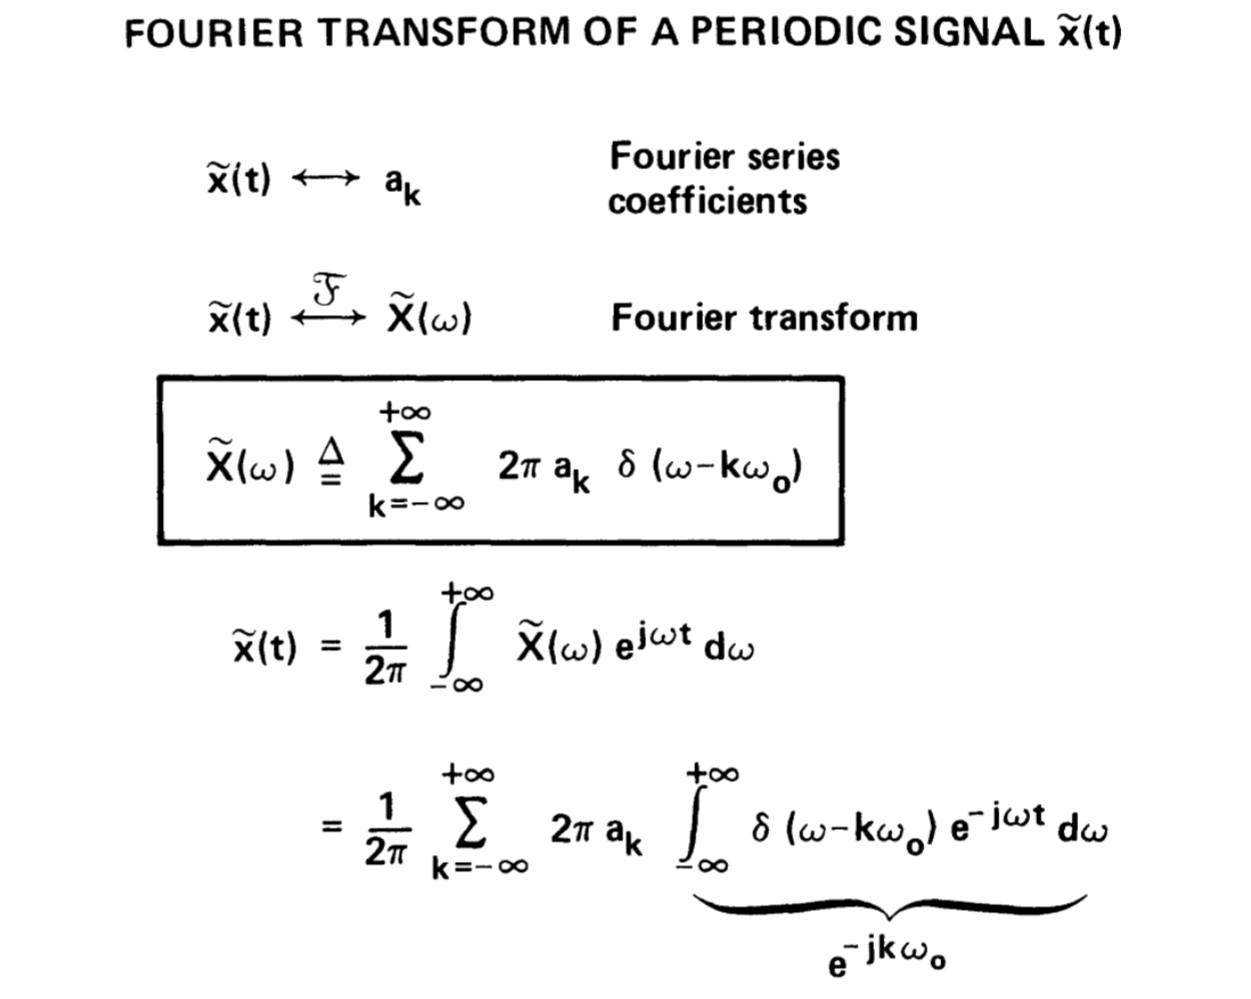
\includegraphics[width=0.7\linewidth]{FSvsFT}
    \end{figure}
\end{frame}

\begin{frame}
    \frametitle{FS vs FT: for periodic signal - Example}
    \begin{figure}
        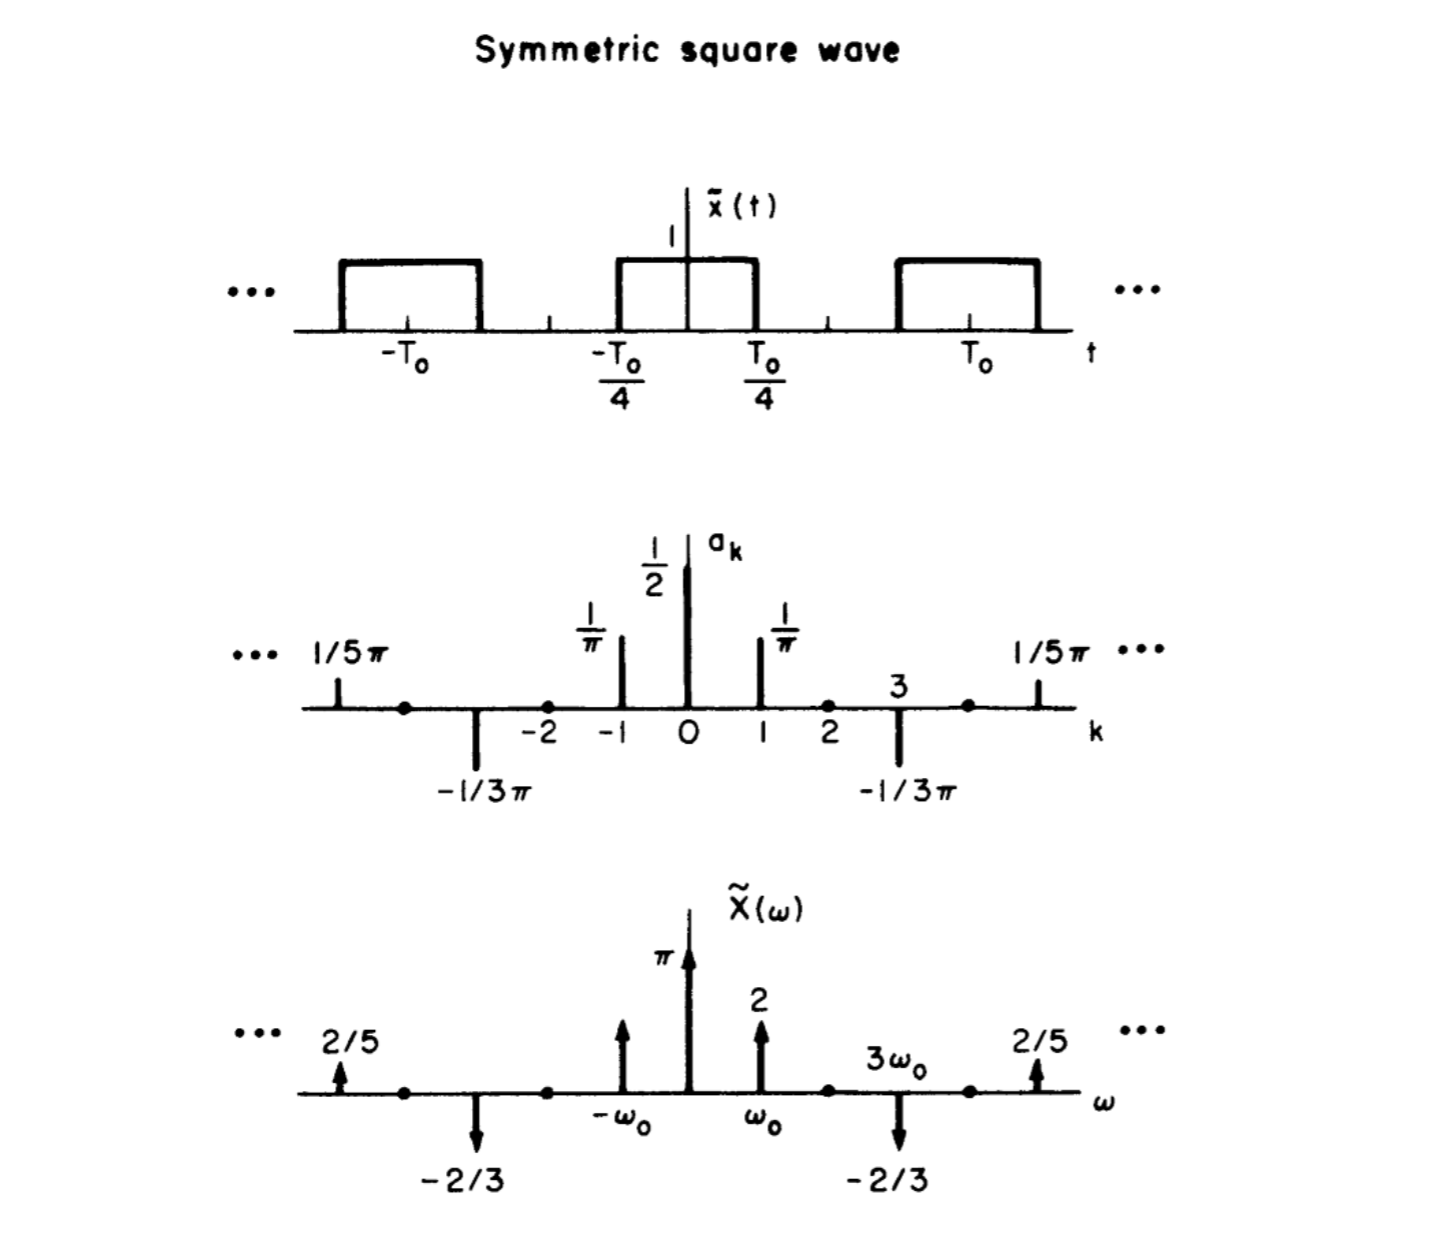
\includegraphics[width=0.7\linewidth]{FSvsFT_eg}
    \end{figure}
\end{frame}



\begin{frame}
    \frametitle{FS vs FT: definition}
    Fourier Series: for periodic signals
    \begin{figure}
        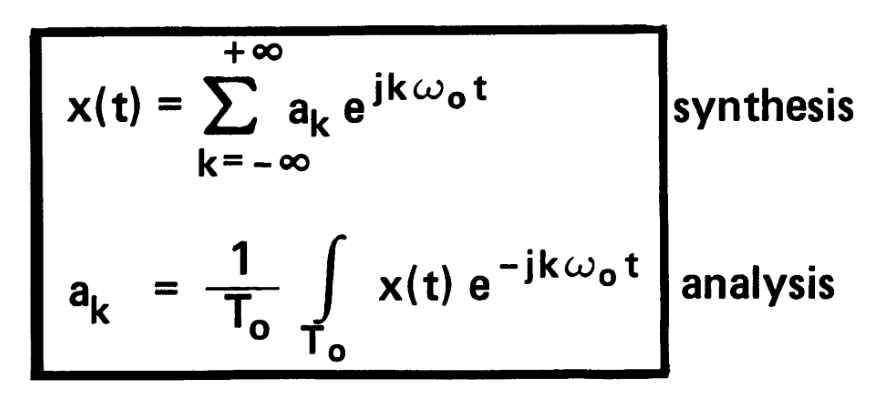
\includegraphics[width=0.4\linewidth]{FS_def}
    \end{figure}
    Fourier Transform: for ``all'' signals, often aperiodic
    \begin{figure}
        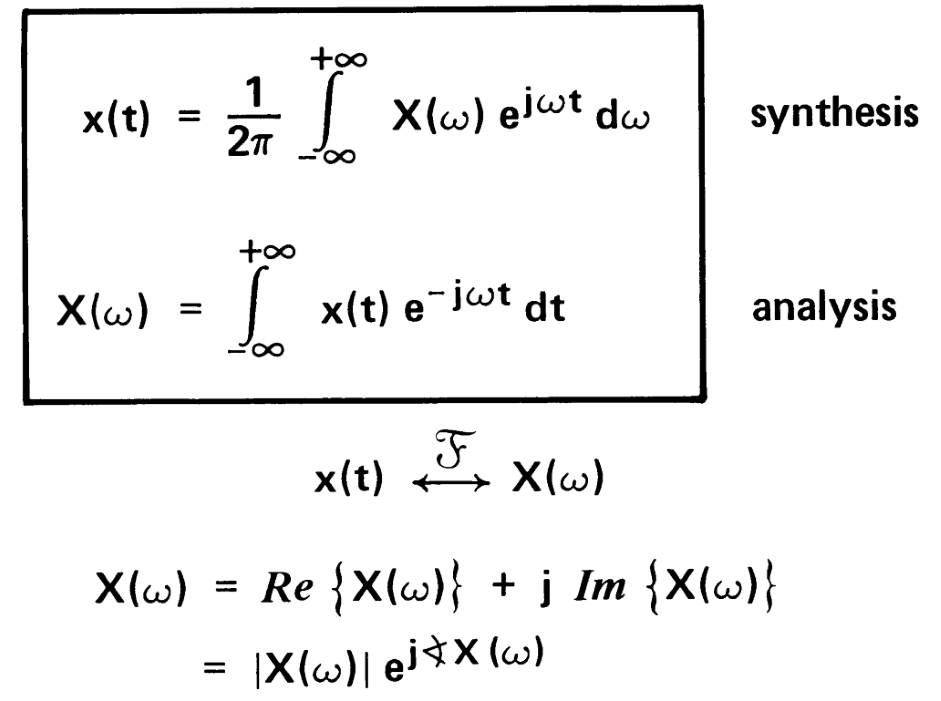
\includegraphics[width=0.4\linewidth]{FT_def}
    \end{figure}
\end{frame}


%------------------------------------------------
\section{Chap.6: Filtering}
%------------------------------------------------
\subsection{FS: Filtering}

\begin{frame}
    \frametitle{FS: Filtering}
Input-Output Relation:
\begin{figure}
    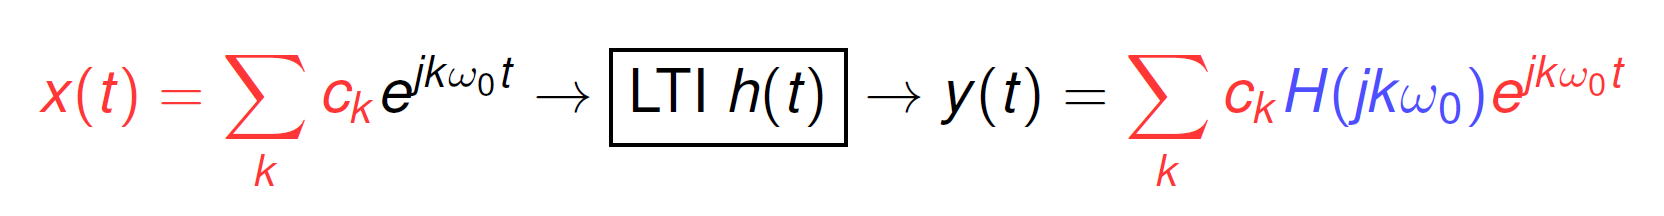
\includegraphics[width=0.6\linewidth]{input_output}
\end{figure}

Example:
\begin{figure}
    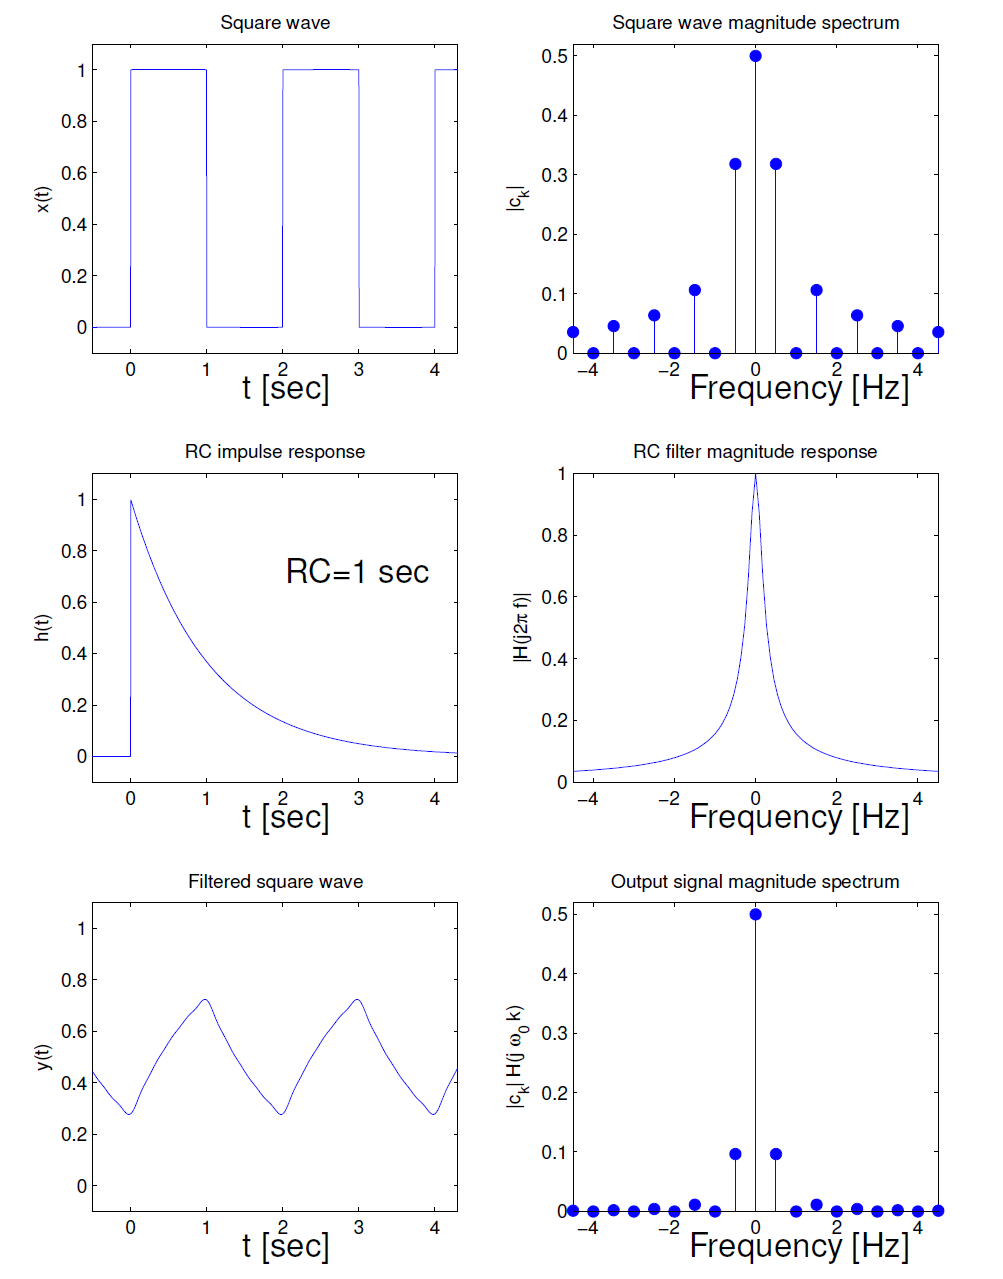
\includegraphics[width=0.35\linewidth]{filter_eg.PNG}
\end{figure}
\end{frame}


\subsection{FT: Filtering}
\begin{frame}
    \frametitle{FT: Filtering}
    \begin{itemize}
    \item Convolution Property: $h(t)* x(t) \stackrel{\mathscr{F}}{\longleftrightarrow} H(\omega) X(\omega)    $
    
    \begin{figure}
    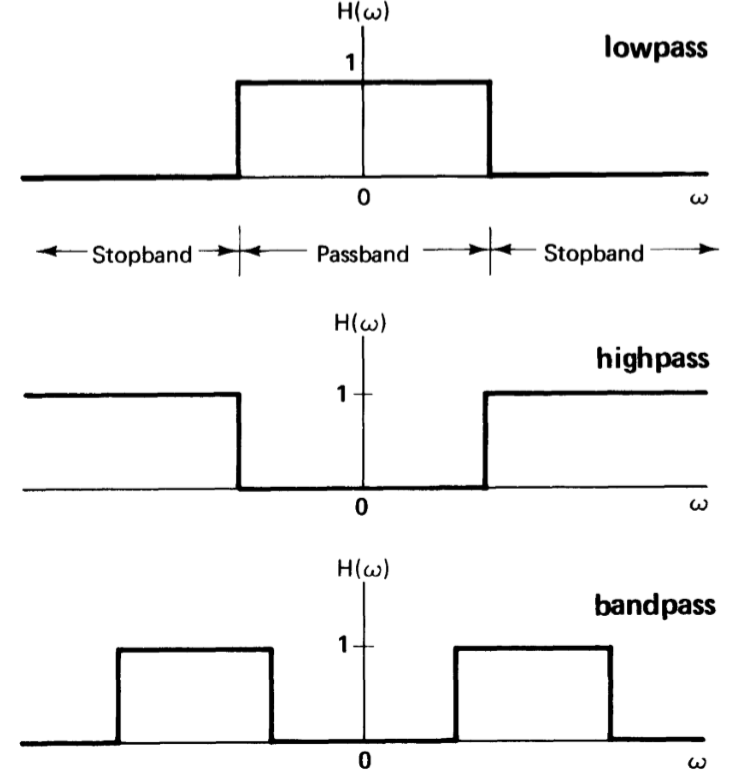
\includegraphics[width=0.5\linewidth]{filter}
    \end{figure}
    \item LTI systems can be viewed as ``filters'' in frequency domain
    \end{itemize}
\end{frame}

\begin{frame}[t]
    \frametitle{Lowpass Filter}
    \begin{figure}
        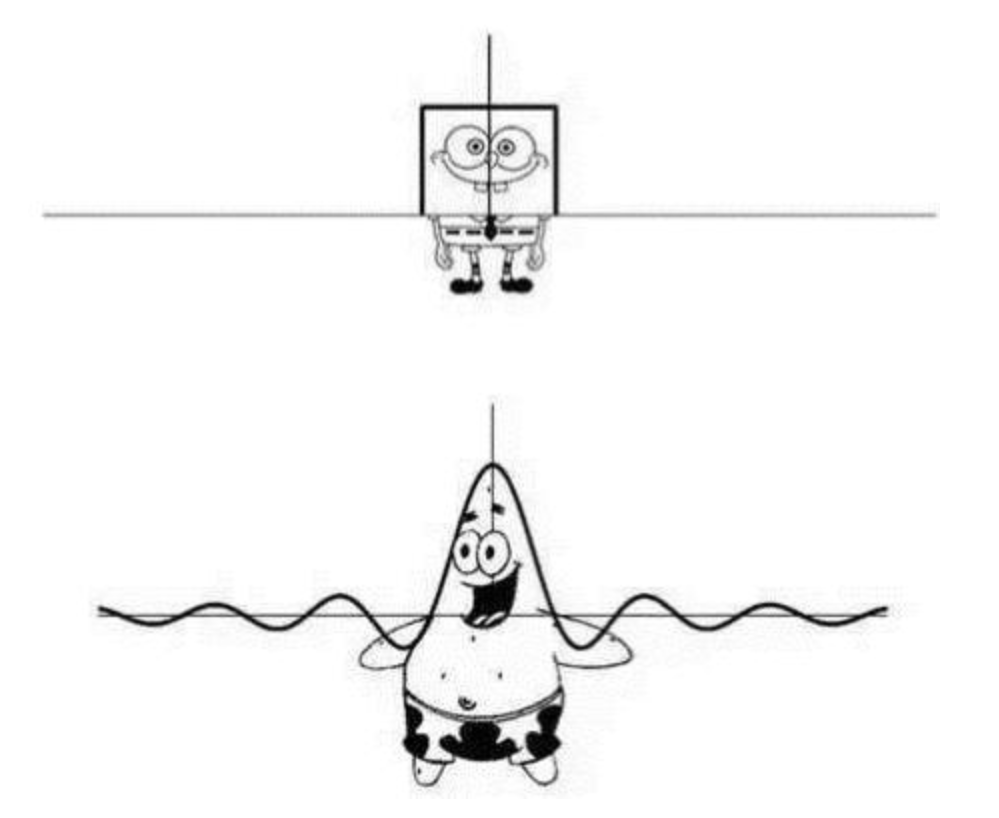
\includegraphics[width=0.4\linewidth]{sponge.PNG}
    \end{figure}
    \begin{center}
        \begin{align*}
            \text{Patrick Star} &\stackrel{FT}{\longleftrightarrow} \text{SpongeBob SquarePants}    \\[1em]          
        \end{align*}
    \end{center} 
\end{frame}



\begin{frame}[t]
    \frametitle{Exercise: FS Filtering - HW3 Q11}
    \begin{figure}
        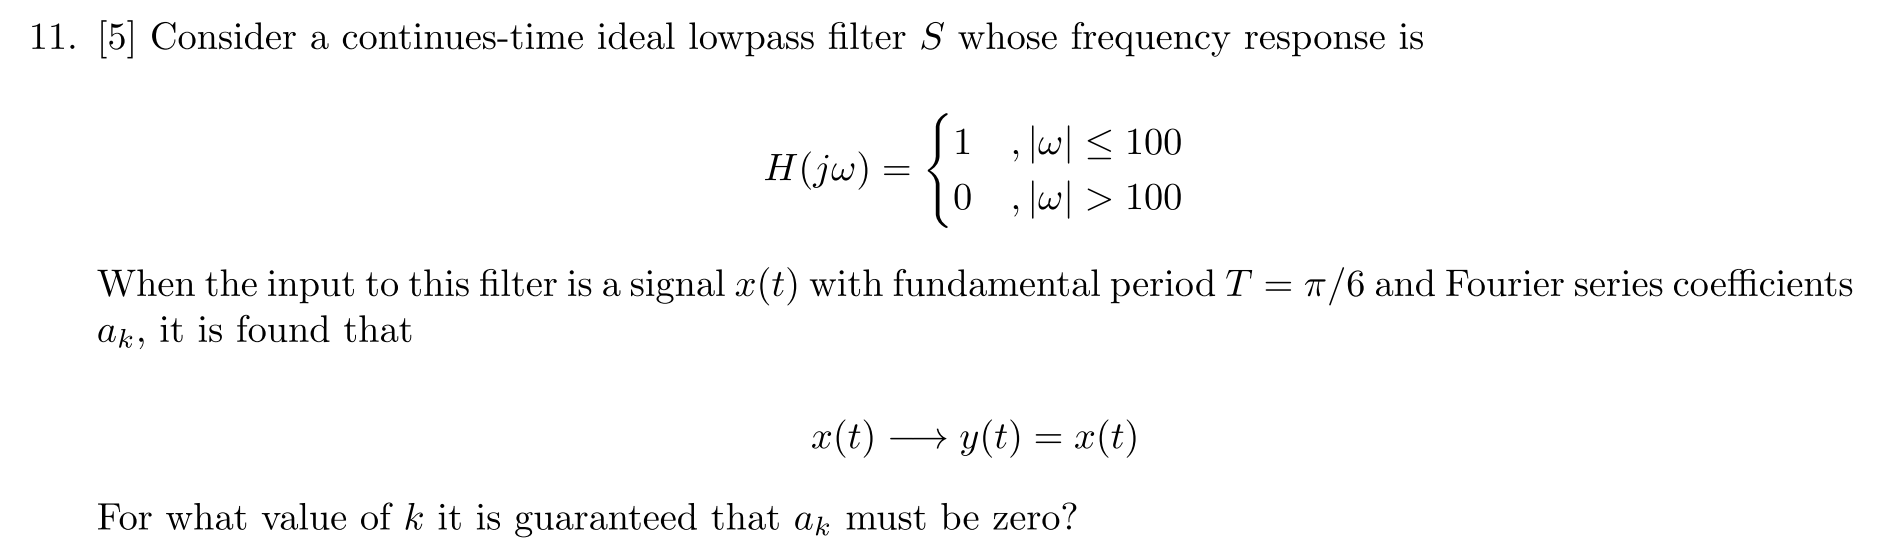
\includegraphics[width=1\linewidth]{hw3_q11}
    \end{figure}
\end{frame}



\begin{frame}[t]
    \frametitle{Exercise - FT: Filtering}
    \begin{figure}
        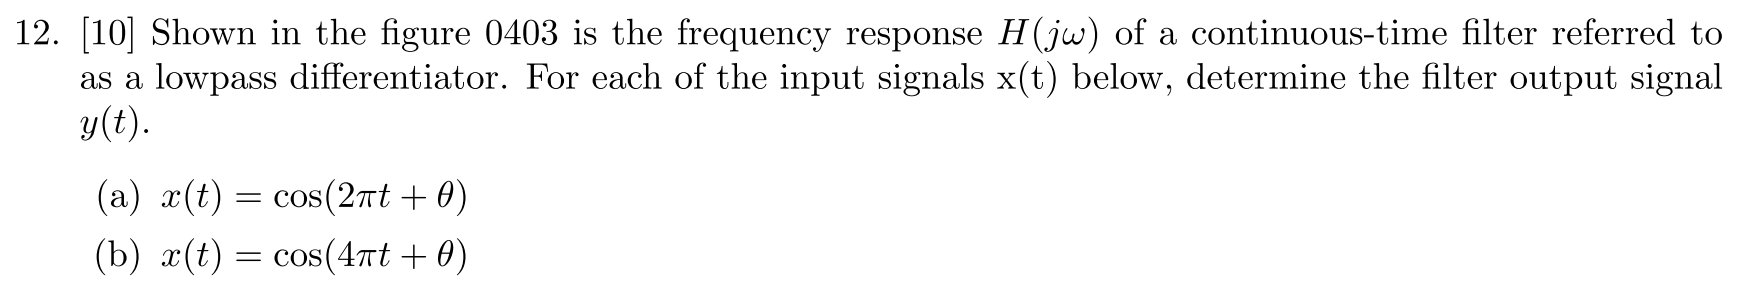
\includegraphics[width=1\linewidth]{q12a}
    \end{figure}
    \begin{figure}
        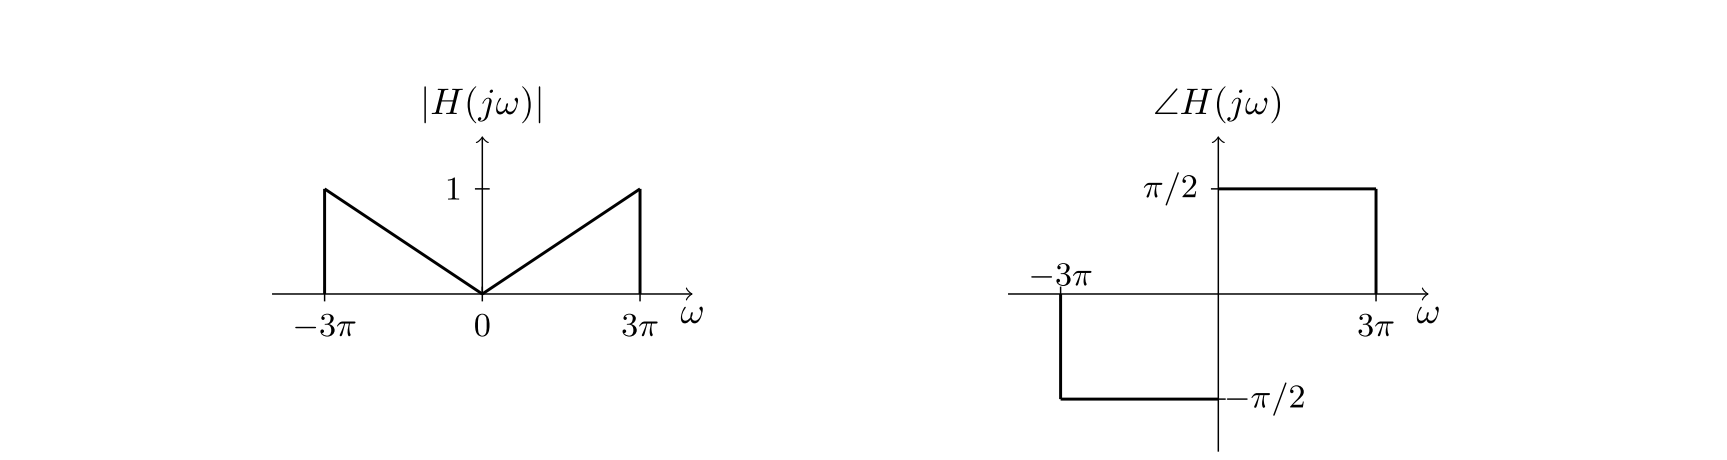
\includegraphics[width=1\linewidth]{q12b}
    \end{figure}
    Hint:
    \begin{figure}
        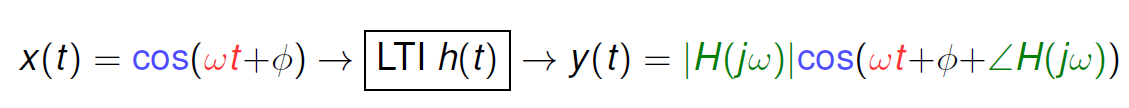
\includegraphics[width=0.8\linewidth]{cosin_cosout}
    \end{figure}
 
\end{frame}

\begin{frame}[t]
    \frametitle{Exercise - FT: Filtering}
    \begin{figure}
        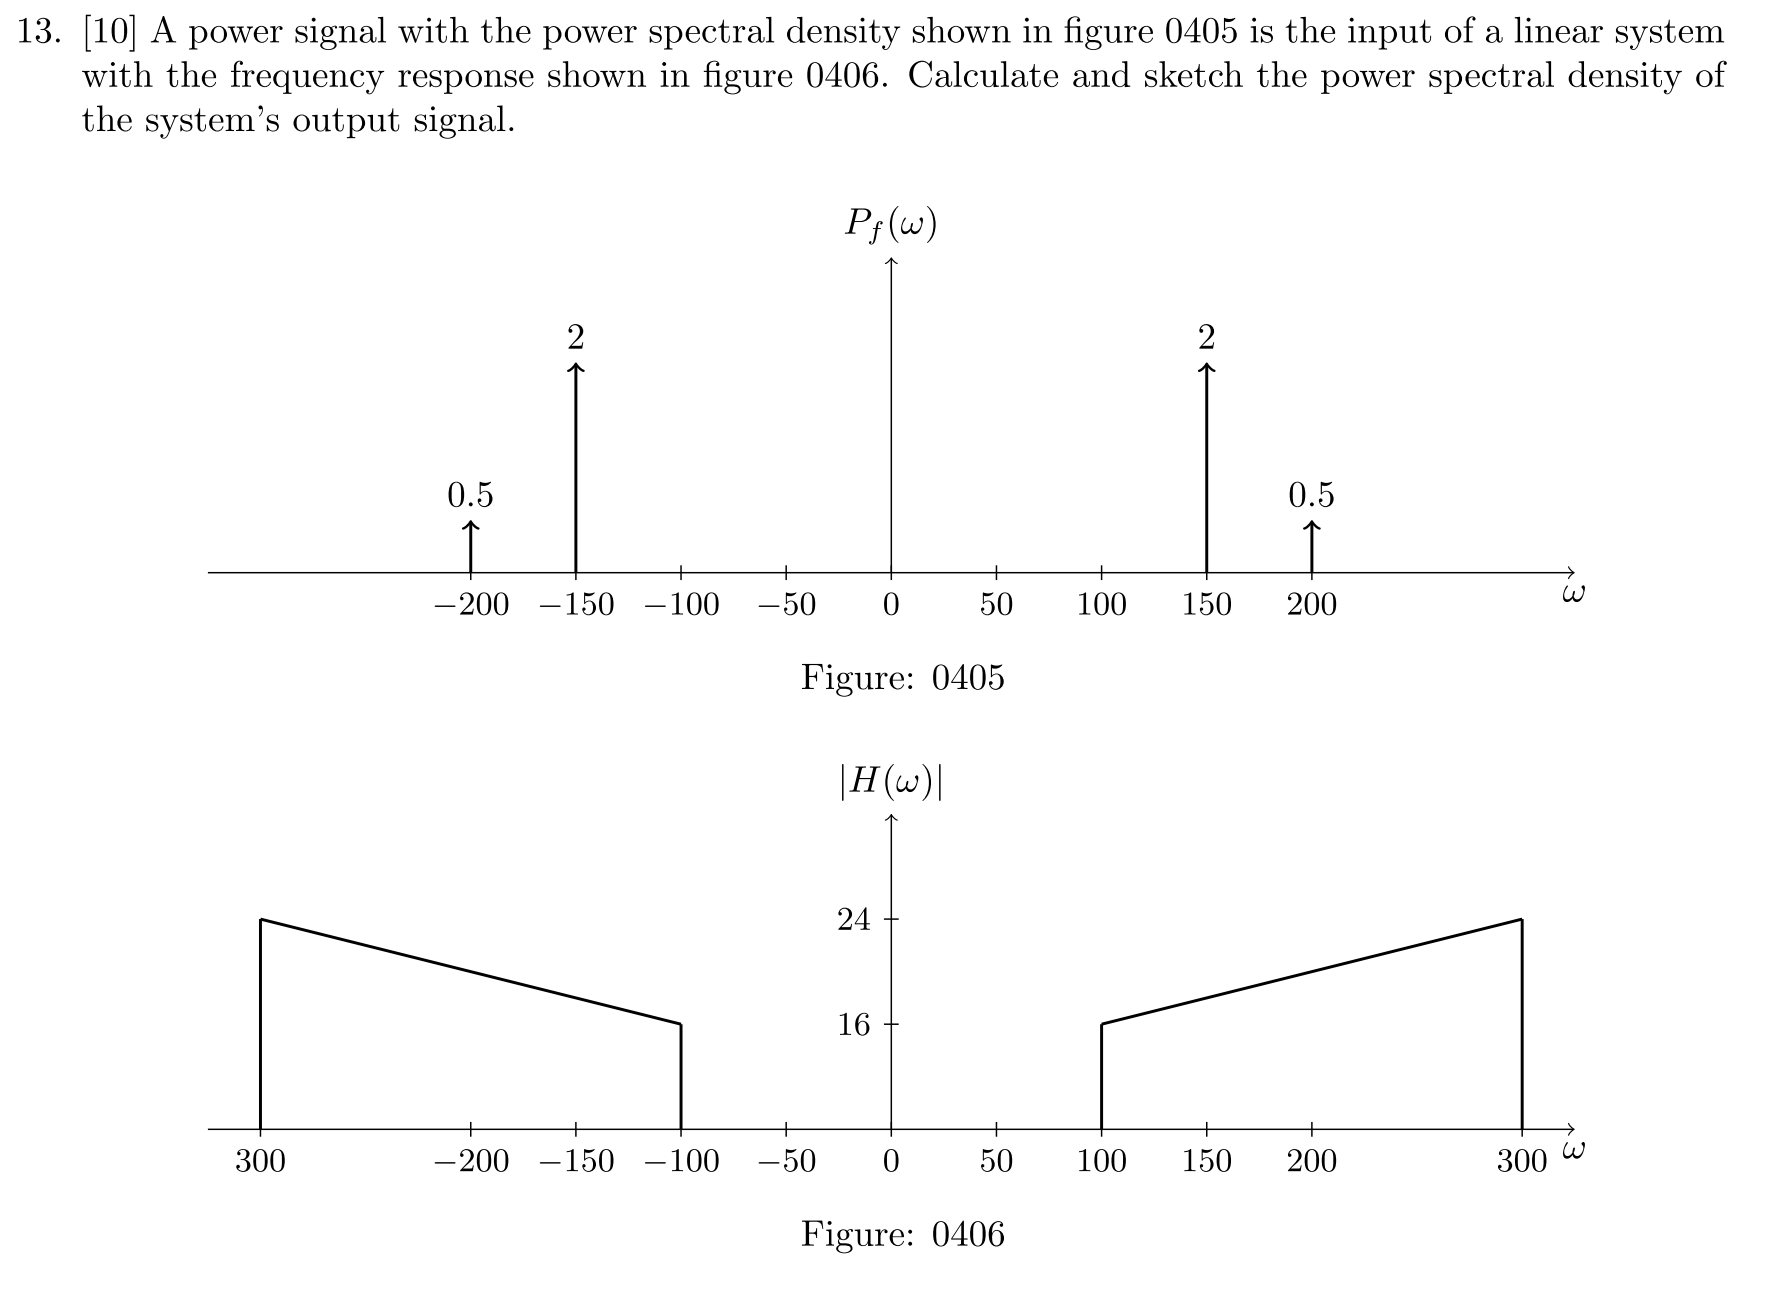
\includegraphics[width=0.8\linewidth]{q13}
    \end{figure}

\end{frame}



\section{Summary}
\begin{frame}
    \frametitle{Summary}
    \begin{itemize}
        \item FS vs FT
        \item Physical meaning of FT
        \item The place we are in the big picture
        \item For Filtering
        \begin{itemize}
            \item if want y(t), then using FS is easier
            \item for FT, it is more elegant: we are either in time domain or freq. domain
        \end{itemize}
    \end{itemize}
\end{frame}

%------------------------------------------------

\begin{frame}
\Huge{\centerline{The End}}
\end{frame}

%----------------------------------------------------------------------------------------

\end{document} 